\PassOptionsToPackage{unicode=true}{hyperref} % options for packages loaded elsewhere
\PassOptionsToPackage{hyphens}{url}
%
\documentclass[12pt,a4paper,twoside]{article}
\usepackage{lmodern}
\usepackage{setspace}
\setstretch{1.2}
\usepackage{amssymb,amsmath}
\usepackage{ifxetex,ifluatex}
\usepackage{fixltx2e} % provides \textsubscript
\ifnum 0\ifxetex 1\fi\ifluatex 1\fi=0 % if pdftex
  \usepackage[T1]{fontenc}
  \usepackage[utf8]{inputenc}
  \usepackage{textcomp} % provides euro and other symbols
\else % if luatex or xelatex
  \usepackage{unicode-math}
  \defaultfontfeatures{Ligatures=TeX,Scale=MatchLowercase}
\fi
% use upquote if available, for straight quotes in verbatim environments
\IfFileExists{upquote.sty}{\usepackage{upquote}}{}
% use microtype if available
\IfFileExists{microtype.sty}{%
\usepackage[]{microtype}
\UseMicrotypeSet[protrusion]{basicmath} % disable protrusion for tt fonts
}{}
\IfFileExists{parskip.sty}{%
\usepackage{parskip}
}{% else
\setlength{\parindent}{0pt}
\setlength{\parskip}{6pt plus 2pt minus 1pt}
}
\usepackage{hyperref}
\hypersetup{
            pdftitle={Reproducibility made simple},
            pdfauthor={Aaron Peikert},
            pdfborder={0 0 0},
            breaklinks=true}
\urlstyle{same}  % don't use monospace font for urls
\usepackage[left=4cm, right=3cm, top=2.5cm, bottom=2.5cm]{geometry}
\usepackage{color}
\usepackage{fancyvrb}
\newcommand{\VerbBar}{|}
\newcommand{\VERB}{\Verb[commandchars=\\\{\}]}
\DefineVerbatimEnvironment{Highlighting}{Verbatim}{commandchars=\\\{\}}
% Add ',fontsize=\small' for more characters per line
\usepackage{framed}
\definecolor{shadecolor}{RGB}{248,248,248}
\newenvironment{Shaded}{\begin{snugshade}}{\end{snugshade}}
\newcommand{\AlertTok}[1]{\textcolor[rgb]{0.94,0.16,0.16}{#1}}
\newcommand{\AnnotationTok}[1]{\textcolor[rgb]{0.56,0.35,0.01}{\textbf{\textit{#1}}}}
\newcommand{\AttributeTok}[1]{\textcolor[rgb]{0.77,0.63,0.00}{#1}}
\newcommand{\BaseNTok}[1]{\textcolor[rgb]{0.00,0.00,0.81}{#1}}
\newcommand{\BuiltInTok}[1]{#1}
\newcommand{\CharTok}[1]{\textcolor[rgb]{0.31,0.60,0.02}{#1}}
\newcommand{\CommentTok}[1]{\textcolor[rgb]{0.56,0.35,0.01}{\textit{#1}}}
\newcommand{\CommentVarTok}[1]{\textcolor[rgb]{0.56,0.35,0.01}{\textbf{\textit{#1}}}}
\newcommand{\ConstantTok}[1]{\textcolor[rgb]{0.00,0.00,0.00}{#1}}
\newcommand{\ControlFlowTok}[1]{\textcolor[rgb]{0.13,0.29,0.53}{\textbf{#1}}}
\newcommand{\DataTypeTok}[1]{\textcolor[rgb]{0.13,0.29,0.53}{#1}}
\newcommand{\DecValTok}[1]{\textcolor[rgb]{0.00,0.00,0.81}{#1}}
\newcommand{\DocumentationTok}[1]{\textcolor[rgb]{0.56,0.35,0.01}{\textbf{\textit{#1}}}}
\newcommand{\ErrorTok}[1]{\textcolor[rgb]{0.64,0.00,0.00}{\textbf{#1}}}
\newcommand{\ExtensionTok}[1]{#1}
\newcommand{\FloatTok}[1]{\textcolor[rgb]{0.00,0.00,0.81}{#1}}
\newcommand{\FunctionTok}[1]{\textcolor[rgb]{0.00,0.00,0.00}{#1}}
\newcommand{\ImportTok}[1]{#1}
\newcommand{\InformationTok}[1]{\textcolor[rgb]{0.56,0.35,0.01}{\textbf{\textit{#1}}}}
\newcommand{\KeywordTok}[1]{\textcolor[rgb]{0.13,0.29,0.53}{\textbf{#1}}}
\newcommand{\NormalTok}[1]{#1}
\newcommand{\OperatorTok}[1]{\textcolor[rgb]{0.81,0.36,0.00}{\textbf{#1}}}
\newcommand{\OtherTok}[1]{\textcolor[rgb]{0.56,0.35,0.01}{#1}}
\newcommand{\PreprocessorTok}[1]{\textcolor[rgb]{0.56,0.35,0.01}{\textit{#1}}}
\newcommand{\RegionMarkerTok}[1]{#1}
\newcommand{\SpecialCharTok}[1]{\textcolor[rgb]{0.00,0.00,0.00}{#1}}
\newcommand{\SpecialStringTok}[1]{\textcolor[rgb]{0.31,0.60,0.02}{#1}}
\newcommand{\StringTok}[1]{\textcolor[rgb]{0.31,0.60,0.02}{#1}}
\newcommand{\VariableTok}[1]{\textcolor[rgb]{0.00,0.00,0.00}{#1}}
\newcommand{\VerbatimStringTok}[1]{\textcolor[rgb]{0.31,0.60,0.02}{#1}}
\newcommand{\WarningTok}[1]{\textcolor[rgb]{0.56,0.35,0.01}{\textbf{\textit{#1}}}}
\usepackage{longtable,booktabs}
% Fix footnotes in tables (requires footnote package)
\IfFileExists{footnote.sty}{\usepackage{footnote}\makesavenoteenv{longtable}}{}
\usepackage{graphicx,grffile}
\makeatletter
\def\maxwidth{\ifdim\Gin@nat@width>\linewidth\linewidth\else\Gin@nat@width\fi}
\def\maxheight{\ifdim\Gin@nat@height>\textheight\textheight\else\Gin@nat@height\fi}
\makeatother
% Scale images if necessary, so that they will not overflow the page
% margins by default, and it is still possible to overwrite the defaults
% using explicit options in \includegraphics[width, height, ...]{}
\setkeys{Gin}{width=\maxwidth,height=\maxheight,keepaspectratio}
\setlength{\emergencystretch}{3em}  % prevent overfull lines
\providecommand{\tightlist}{%
  \setlength{\itemsep}{0pt}\setlength{\parskip}{0pt}}
\setcounter{secnumdepth}{5}
% Redefines (sub)paragraphs to behave more like sections
\ifx\paragraph\undefined\else
\let\oldparagraph\paragraph
\renewcommand{\paragraph}[1]{\oldparagraph{#1}\mbox{}}
\fi
\ifx\subparagraph\undefined\else
\let\oldsubparagraph\subparagraph
\renewcommand{\subparagraph}[1]{\oldsubparagraph{#1}\mbox{}}
\fi

% set default figure placement to htbp
\makeatletter
\def\fps@figure{htbp}
\makeatother

\usepackage{booktabs}
\usepackage{libertine}
\usepackage{libertinust1math}
\usepackage{sourcecodepro}
\usepackage{emptypage}
\usepackage{nopageno}
\renewcommand{\textfraction}{0.05}
\renewcommand{\topfraction}{0.8}
\renewcommand{\bottomfraction}{0.8}
\renewcommand{\floatpagefraction}{0.75}
\DefineVerbatimEnvironment{Highlighting}{Verbatim}{commandchars=\\\{\},fontsize=\footnotesize}
%% change fontsize of output
\let\oldverbatim\verbatim
\let\endoldverbatim\endverbatim
\renewenvironment{verbatim}{\footnotesize\oldverbatim}{\endoldverbatim}
\usepackage{etoolbox}
\makeatletter
\providecommand{\subtitle}[1]{% add subtitle to \maketitle
  \apptocmd{\@title}{\par {\large #1 \par}}{}{}
}
\makeatother

\title{Reproducibility made simple}
\providecommand{\subtitle}[1]{}
\subtitle{Automating reproducible research workflows}
\author{Aaron Peikert}
\date{2020-08-11}

\begin{document}
\maketitle

{
\setcounter{tocdepth}{2}
\tableofcontents
}
\newpage\null\thispagestyle{empty}\newpage

\hypertarget{abstract}{%
\section*{Abstract}\label{abstract}}
\addcontentsline{toc}{section}{Abstract}

This thesis discusses the practical and metascientific merits of reproducibility and presents \href{https://github.com/aaronpeikert/repro}{\texttt{repro}}, an R package which drastically simplifies the adherence to the best practices proposed by Peikert \& Brandmaier (\protect\hyperlink{ref-peikertReproducibleDataAnalysis2019}{2019}).
The resulting workflow complies with open science principles, is transferable across machines and conserved through time.
Consequently, research projects are virtually guaranteed to reproduce and are easier to replicate.
It is explained how the technical solutions, namely Git, RMarkdown, Make, and Docker, overcome common reproducibility problems and how the interaction with these tools is simplified through automation.
The high degree of automation allows the workflow to scale well across researchers, letting them collaborate more transparently and effectively, as well as across machines, utilizing high performance and cloud computing technology.
To adapt to the ever-shifting landscape of software requirements \href{https://github.com/aaronpeikert/repro}{\texttt{repro}} has a modular design allowing other workflow packages to build upon its infrastructure.

\hypertarget{acknowledgements}{%
\section*{Acknowledgements}\label{acknowledgements}}
\addcontentsline{toc}{section}{Acknowledgements}

I dedicate this thesis to my mother, who endured what cannot be described to give what only can be felt.

I want to thank my advisers, Dr.~Andreas M. Brandmaier and Prof.~Manuel Völkle for their time and patience, and my friends for their resourceful advice:

\begin{itemize}
\tightlist
\item
  Jakob Eißner (commits \href{https://github.com/aaronpeikert/repro-thesis/commit/bc53e58cf1861b4dbc4447853ad7f3895dd805ea}{\texttt{bc53e58}}, \href{https://github.com/aaronpeikert/repro-thesis/commit/9841a3695b9bc607b95e06e3d30b45116c6681ab}{\texttt{9841a36}} \& \href{https://github.com/aaronpeikert/repro-thesis/commit/4857dcb8536136efa63bbe5efb2da6ae6fc10681}{\texttt{4857dcb}})
\item
  Elisabeth Riha (commit \href{https://github.com/aaronpeikert/repro-thesis/commit/82f32d4d15dd3014dc0cf847166e0b023ea11a8a}{\texttt{82f32d4}})
\item
  Caroline Gahrmann (commit \href{https://github.com/aaronpeikert/repro-thesis/commit/d9a730cb1bdcedef3312bc2be32ad81a3d2a45b9}{\texttt{d9a730c}})
\end{itemize}

\newpage

\hypertarget{theoretical-considerations}{%
\section{Theoretical Considerations}\label{theoretical-considerations}}

Claerbout \& Karrenbach (\protect\hyperlink{ref-claerboutElectronicDocumentsGive1992}{1992}) define reproducibility as the ability to obtain the same results, from the same dataset.
Conversely, they call a result replicable if one draws the same conclusion from a new dataset.
This thesis concerns itself with the former, providing researchers with an accessible analysis workflow, that is virtually guaranteed to reproduce across time and devices.

The scientific community agrees that ideally their work should be reproducible.
Indeed it may be hard to find a researcher who distrusts a result because it is reproducible; to the contrary, many argue it is ``good scientific practice'' to ensure what they consider reproducible (``Reducing Our Irreproducibility,'' \protect\hyperlink{ref-AnnouncementReducingOur2013}{2013}; Deutsche Forschungsgemeinschaft, \protect\hyperlink{ref-dfg2019}{2019}; Epskamp, \protect\hyperlink{ref-epskamp2019rep}{2019}).
Several reasons, practical and meta-scientific, justify this consensus of reproducibility as a minimal standard of Science.

Reproducibility makes researchers life more productive in two ways:
The act of reproduction provides, at the most basic level, an opportunity for the researcher to spot errors. At the same time, other researchers may also benefit from reusing materials from an analysis they reproduced.

Beyond these two purely pragmatic reasons, reproduction is crucial, depending on the philosophical view of Science one subscribes to, because it allows independent validation and enables replication.
Philosophers of Science characterise Science mainly as a shared method of determining whether or not a statement about the world is ``true'' (Andersen \& Hepburn, \protect\hyperlink{ref-andersonScientificMethod2016}{2016}) or more broadly evaluating the statements verisimilitude (Gilbert, \protect\hyperlink{ref-gilbertModelBuildingDefinition1991}{1991}; Meehl, \protect\hyperlink{ref-meehlAppraisingAmendingTheories1990}{1990}; Popper, \protect\hyperlink{ref-popperCommentsTruthGrowth1962}{1962}; Tichỳ, \protect\hyperlink{ref-tichyVerisimilitudeRedefined1976}{1976}).
If this method is for experts to agree on the assumptions and deduce ``truth'', reproducibility is hardly necessary.
On the other hand, it does gain importance if one induces facts by carefully observing the world.
The decisive difference between the above approaches is that the former gains credibility by the authority of the experts, while the latter is trustworthy because anyone may verify it.

Accepting induction as a scientific method hence hinges on the verifiability by others.
Some have even argued that such democratisation of Science is what fueled the so-called scientific revolution (Heilbron, \protect\hyperlink{ref-heilbronOxfordCompanionHistory2004}{2004}, Scientific Revolution).
The scientific revolution had the experiment as an agreed-upon method to observe reality, and a much later revolution provides statistical modelling (Rodgers, \protect\hyperlink{ref-rodgersEpistemologyMathematicalStatistical2010}{2010}) as a means to induction.
This consensus about how to observe and how to induce gives modern scientific enterprises much of their credibility.
Two reasons justify why we must assume reproducibility as a scientific standard if we accept induction as a scientific method:
First, it enables independent verification of the process of induction, and second, it dramatically simplifies replication as a means to verify the induced truths.

However, neither the practical reasons that results might be less error-prone and more reusable nor that the process of induction and the induced facts are more straightforward to verify, if reproducible, derive strictly from the definition of reproducibility provided by Claerbout \& Karrenbach (\protect\hyperlink{ref-claerboutElectronicDocumentsGive1992}{1992}) given above.
A simple thought experiment illustrates this shortcoming:
Imagine a binary---therefore only machine readable---program being perfectly reproducible; hence upon the input of the same dataset, it fills a scientific manuscript with the same numbers at the right places.
Furthermore, let us assume this hypothetical program may never hold if the dataset changes.
Does the predicate ``reproducible'' in this situation reduce the number of mistakes or enables reuse? Unlikely.
Or could one audit it and use it in replication? Hardly.
This admittedly constructed case of a reproducible black box shows that we are not interested in reproducibility but rather in its side effects.
Because it is a binary programm, it does not enhance understanding and because it not applicable to other datasets, it does not facilitate productivity.
In fact such program does not grant the researcher any practical nor metascientific advantages over non-reproducible research products.

Spoiling its elegant simplicity, I extend the definition by Claerbout \& Karrenbach (\protect\hyperlink{ref-claerboutElectronicDocumentsGive1992}{1992}) to address this issue, by further demanding that reproducibility must facilitate replication.
Hence, I would only call a result reproducible if the results remain unchanged if the data does, and it furthermore helps other researchers to replicate the results if they attempt to.
With such a notion, the only valid cause of reproducibility is transparency.
Only if it is clear how data relates to its results, both reproducibility and replication get promoted.
Consequently, something is no longer either reproducible or not, but there are shades because a research product can promote replication to varying degrees.
Note that a scientific result can facilitate replication without anyone ever attempting to replicate it, e.g.~by educating other researchers about the analyses method, being openly accessible and providing reusable components.

Hence, reproducibility has a technical side, which is ensuring the same results, and a non-technical side, which is facilitating understanding.
The former relates to the practical advantages while the latter serves the metascientific purposes of reproducibility.
An important caveat of the technical aspect is that generating the same results from the same data should always be possible regardless of time and machine.
As such, a reproducible analysis should be:

\begin{enumerate}
\def\labelenumi{\arabic{enumi}.}
\tightlist
\item
  understandable by other researchers,
\item
  transferable across machines,
\item
  conserved through time.
\end{enumerate}

This much more demanding standard of reproducibility is justified by two recent developments in the social sciences in general and psychology in particular: the emergence of a ``replication crises'' (Ioannidis, \protect\hyperlink{ref-ioannidisWhyMostPublished2005}{2005}) and the rise of ``machine learning'' (Jordan \& Mitchell, \protect\hyperlink{ref-jordanMachineLearningTrends2015}{2015}) as a scientific tool.
Both trends link to the use of statistical modelling on which the social sciences became reliant for testing and developing their theories (Gigerenzer et al., \protect\hyperlink{ref-gigerenzerNullRitualWhat2004}{2004}; Meehl, \protect\hyperlink{ref-meehlTheoreticalRisksTabular1978}{1978}).
It turns out that, if one fits the very same statistical model as published on newly gathered data, one fails more often to achieve the same results as published then one succeeds. (Open Science Collaboration, \protect\hyperlink{ref-opensciencecollaborationEstimatingReproducibilityPsychological2015}{2015}).

Such failure to replicate findings that were believed to be robust has grown to a level that some social scientists call a crisis.
They put forth various causes and remedies to this crisis.
Most remedies share a common motif: transparency.
Some call for Bayesian statistics (Maxwell et al., \protect\hyperlink{ref-maxwellPsychologySufferingReplication2015}{2015}), as it makes assumptions more explicit, or demand preregistration (Nosek et al., \protect\hyperlink{ref-nosekPreregistrationRevolution2018}{2018}) as a means to clarify how to analyse the data, beforehand and publicly. Others require the researchers to publish their data (Boulton et al., \protect\hyperlink{ref-boultonScienceOpenEnterprise2012}{2012}).
Similar calls for transparency, as a response to the replication crises, have formed the open science movement which stresses the necessity of six principles (Kraker et al., \protect\hyperlink{ref-krakerCaseOpenScience2011}{2011}):

\begin{itemize}
\tightlist
\item
  Open Access,
\item
  Open Data,
\item
  Open Source,
\item
  Open Methodology,
\item
  Open Peer Review and
\item
  Open Educational Resources.
\end{itemize}

I argue that a research product resting on these pillars facilitates replication optimally and hence, it satisfies the highest standard of reproducibility.
If everyone has access to a scientific product and its data along with the source code, everyone has the possibility of understanding the underlying methodology, which enables them to criticise the results and educate themselves.
Having done so, they are in the best position for replication.
Hence, any one's ability to reproduce such a result gives a tangible affirmation of its usefulness to the scientific community.

While reproducibility is no hurdle if one can perform the calculations needed with a pocket calculator, the more and more frequent use of computer-intensive methods renders such expectation questionable.
The use of machine learning techniques, which has been once enabled by the computer taking over strenuous works, now impedes our quest for reproducibility.
More massive amounts of more complicated computer code than ever before create room for errors and misunderstandings, leading the machine learning community to believe that they face a reproducibility crisis themselves (Hutson, \protect\hyperlink{ref-hutsonArtificialIntelligenceFaces2018}{2018}).
Yet, I am far from calling for abstinence from machine learning, just because it complicates reproduction, but want to emphasise the need for solutions that allow anyone to reproduce even the most sophisticated analysis.

Peikert \& Brandmaier (\protect\hyperlink{ref-peikertReproducibleDataAnalysis2019}{2019}) put forth an analysis workflow which provides this accessibility for everyone to reproduce any kind of analysis.
However, they fail to provide the same level of convenience for the researcher who created an analysis in the first place.
Setting up the workflow eats up a considerable amount of the researcher's time, which they may rather spend on advancing research.
This additional effort offsets the increase in productivity, promised by reproducibility, which I regard as most significant in the workflows adoption.
Persuading researchers, who find the meta-scientific argumentation noble but impractical, do not care about it or even oppose it, requires concrete, practical benefits.
Luckily, most of this setup process may become automated, letting the researcher enjoy the workflows advantages while decreasing the efforts necessary to achieve them.
Providing a version of the analysis workflow by Peikert \& Brandmaier (\protect\hyperlink{ref-peikertReproducibleDataAnalysis2019}{2019}) that is easier to use and more accessible is the goal of this thesis and the herein presented \texttt{repro}-package for the R programming language (Peikert et al., \protect\hyperlink{ref-R-repro}{2020}).

\hypertarget{technical-solutions}{%
\section{Technical Solutions}\label{technical-solutions}}

This section summarises the workflow proposed by Peikert \& Brandmaier (\protect\hyperlink{ref-peikertReproducibleDataAnalysis2019}{2019}; see also The Turing Way Community et al., \protect\hyperlink{ref-theturingwaycommunityTuringWayHandbook2019}{2019} for a very similar approach).
They argue that publicly sharing code is not sufficient to ensure reproducibility:
Instead, reproducibility has to rest on five pillars:

\begin{enumerate}
\def\labelenumi{\arabic{enumi}.}
\item
  \begin{description}
  \tightlist
  \item[file management]
  a folder containing all files, referring to each other using relative paths
  \end{description}
\item
  \begin{description}
  \tightlist
  \item[literate programming]
  a central dynamic document, that relates code to thought
  \end{description}
\item
  \begin{description}
  \tightlist
  \item[version control]
  a system in place that manages revisions of all files over time
  \end{description}
\item
  \begin{description}
  \tightlist
  \item[dependency management]
  a formal description of how files relate to each other
  \end{description}
\item
  \begin{description}
  \tightlist
  \item[containerisation]
  an exact specification of the computational environment
  \end{description}
\end{enumerate}

These pillars stipulate the relations between thought, code and data with their change over time and environment and hence, they reach all requirements of reproducibility through being:

\begin{enumerate}
\def\labelenumi{\arabic{enumi}.}
\tightlist
\item
  understandable to other researchers,
\item
  transferable across machines,
\item
  conserved through time.
\end{enumerate}

While comprehensibility to the scientific community is probably the most crucial objective, it is also the most difficult to achieve.
That is because as a non-technical requirement, no set of rules can assure its fulfilment (though clear writing\footnote{Williams (\protect\hyperlink{ref-williamsStyleLessonsClarity2017}{2017}) provides some excellent principles for writing clearly.} and clean code\footnote{Martin (\protect\hyperlink{ref-martinCleanCoderCode2011}{2011}) proposes a coding paradigm that found widespread use because of its focus on understandability.} certainly help).
Transfer and conservation, on the other hand, are problems with technical solutions.

Peikert \& Brandmaier (\protect\hyperlink{ref-peikertReproducibleDataAnalysis2019}{2019}) propose to use a combination of RMarkdown, Git, Make, and Docker, because they are the most popular tools for users of the R programming language (R Core Team, \protect\hyperlink{ref-R-base}{2020}) and provide the high-level overview which can be seen in Figure \ref{fig:nutshell}.

\begin{figure}

{\centering \includegraphics[width=1\linewidth]{images/nutshell} 

}

\caption{Overview of the interplay of RMarkdown, Git, Make, and Docker}\label{fig:nutshell}
\end{figure}

However, they stress that any combination of tools is suitable as long as it facilitates the above pillars.

Each of the following sections first raises a challenge for reproducibility, then outlines a conceptual remedy along with a concrete tool and concludes how they relate to the package \texttt{repro}. The relation of these tools with \texttt{repro} is then expanded in the next chapter.

\hypertarget{file-organisation}{%
\subsection{File Organisation}\label{file-organisation}}

File organisation has to meet two challenges: First, the structure needs to be understandable for others, and second, it needs to be self-contained so that it can be moved to another machine.

Adhering to conventions can help other people understand how files are organised.
For example, the filename \texttt{R/reshape.R} both follows standard naming conventions (i.e.~all lowercase; ends with .R; placed within the R directory) and is meaningful. Contrarily, \texttt{myScripts/munge\_Data.r} is probably a lot harder both to understand and to remember for most R-users.

Following two guidelines makes the file structure self-contained:

\begin{enumerate}
\def\labelenumi{\arabic{enumi}.}
\tightlist
\item
  Everything is in one folder.
\item
  Every path is relative to that folder.
\end{enumerate}

This simple concept of a self-contained folder is facilitated by two R specific tools: \href{https://r4ds.had.co.nz/workflow-projects.html}{RStudio projects} and the \texttt{here} package (Müller, \protect\hyperlink{ref-R-here}{2017}).
The former exempts the user from changing the working directory manually; the latter infers absolute paths from relative ones.
However, unlike the native R solution, this inference is consistent across operating systems, scripts and RMarkdowns.

The \texttt{repro} package offers a template for an RStudio Project, which sets up a file structure that follows best practices and conventions.
This template provides the researcher with a minimal example of a reproducible analysis.
The researcher can thus adept code and files to their need, either by merely changing them manually or by the modular structure of \texttt{repro}.

\hypertarget{dynamic-document-generation}{%
\subsection{Dynamic Document Generation}\label{dynamic-document-generation}}

A clear file structure helps researchers to better understand how a scientific analysis relates to the code but an otherwise strict segregation of code and document inhibits a full grasp.
Providing a direct link, dynamic document generation allows interspersing text with code and its results, in order to produce a human-readable document.
The key feature is that every time such a document is rerun, the results are reproduced dynamically.
This functionality eliminates errors due to copy and paste results from statistical software to a text processor. This mistake happens far too often; Nuijten et al. (\protect\hyperlink{ref-nuijtenPrevalenceStatisticalReporting2016}{2016}) reports that 50\% of papers from the psychological sciences contain an error that could have been prevented.

RMarkdown provides a convenient framework to write such dynamic documents and render them as a wide range of output formats\footnote{The document you are viewing also results from a collection of \href{https://github.com/aaronpeikert/repro-thesis}{RMarkdowns} available as \href{https://aaronpeikert.github.io/repro-thesis/}{website}, \href{https://aaronpeikert.github.io/repro-thesis/ma.pdf}{PDF} and \href{https://aaronpeikert.github.io/repro-thesis/ma.epub}{E-book}}. In an RMarkdown, three parts can be distinguished:

\begin{itemize}
\tightlist
\item
  one specifying its output and metadata,
\item
  one containing code, and
\item
  one with descriptive text.
\end{itemize}

Each part uses its own language, all of them designed with ease of use and readability in mind.
The one section containing the output format and other metadata alongside is written in YAML (see the example below).
This specification is located on the top, separated by three dashes at the beginning and at the end of the section.
(R-)Code executing an analysis can be placed in a distinct chunk or inline within the text.
The former has three backticks on their own line signifying beginning and end.
The latter is quoted in a pair single backticks.
Examples of both methods can be found below.
Text which is not fenced by either three dashes or backticks is interpreted as literal text written in the Markup language ``Markdown''.
Markdown allows annotating text to signify formatting like bold, italic, links and the inclusion of images.
This markup is designed to be well readable even as source files.

The following section shows examples of metadata, code and text, specified as above described, forming a minimal example of an RMarkdown (\href{https://github.com/rstudio/rmarkdown-book/blob/a10b33d47a2b223a8ef643c245d45e4dfc7091b8/02-basics.Rmd\#L15-L39}{adapted source code} from Xie et al. (\protect\hyperlink{ref-xieMarkdownDefinitiveGuide2019}{2019})/\href{https://creativecommons.org/licenses/by-nc-sa/4.0/}{CC BY-NC-SA 4.0}):

\begin{Shaded}
\begin{Highlighting}[]
\OtherTok{---}
\FunctionTok{title:}\AttributeTok{ }\StringTok{"Hello R Markdown"}
\FunctionTok{author:}\AttributeTok{ }\StringTok{"Ross Ihaka & Robert Gentleman"}
\FunctionTok{date:}\AttributeTok{ }\StringTok{"1997-04-23"}
\FunctionTok{output:}\AttributeTok{ pdf_document}
\OtherTok{---}
\end{Highlighting}
\end{Shaded}

\begin{Shaded}
\begin{Highlighting}[]
\NormalTok{This is a paragraph in an R Markdown document.}

\NormalTok{Below is a code chunk:}

\BaseNTok{```\{r\}}
\BaseNTok{fit = lm(dist ~ speed, data = cars)}
\BaseNTok{b   = coef(fit)}
\BaseNTok{plot(cars)}
\BaseNTok{abline(fit)}
\BaseNTok{```}

\NormalTok{The slope of the regression is }\BaseNTok{`r b[1]`}\NormalTok{.}
\end{Highlighting}
\end{Shaded}

Resulting in the document seen in Figure \ref{fig:rmarkdown}:

\begin{figure}

{\centering 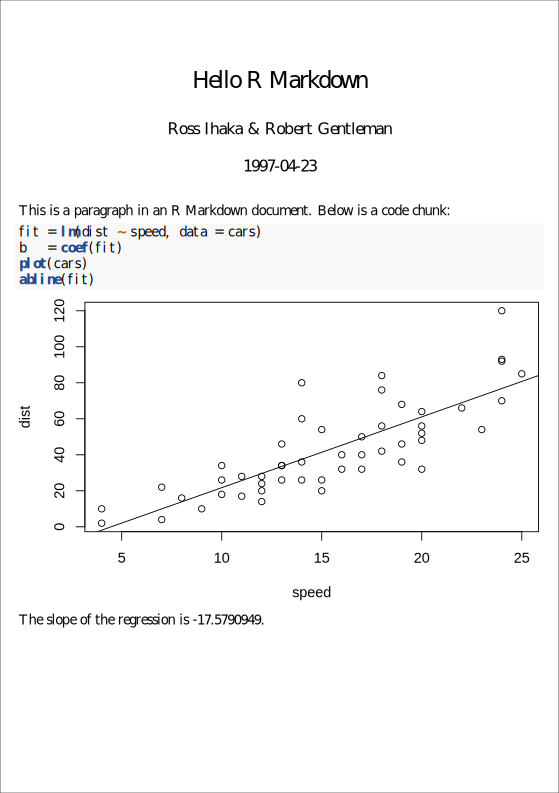
\includegraphics[width=1\linewidth]{images/rmarkdown} 

}

\caption{Result of minimal RMarkdown example.}\label{fig:rmarkdown}
\end{figure}

Undeniably, RMarkdown facilitates reproducibility greatly, but it cannot ensure reproduction. To virtually guarantee reproduction, the \texttt{repro} package extends the YAML metadata to incorporate \protect\hyperlink{dependency-management}{Dependency Management} and \protect\hyperlink{containerisation}{Containerisation} into the process of dynamic document creation.

\hypertarget{version-control}{%
\subsection{Version Control}\label{version-control}}

Text, code and results of a scientific document are refined in cycles of many revisions to accommodate highest standards.
As changes accumulate, different versions do so as well, posing a problem for reproducibility as it may be challenging to find out which version of code relates to the final product.
One may argue that in the typical publication process, the final product is apparent: the published paper.
However, reproducibility may be crucial even before publication as part of collaboration and within the peer-review process.
Also, recent trends in the publication process as preprints, open review, registered reports and post-publication review, blur the lines between published and unpublished.

To organise different versions as changes accumulate across the phases of a project across machines and users is a well-known challenge in software development.
This challenge is met by a high degree of automation that keeps track of different versions and has advanced facilities to compare and merge them.

One such version control software is Git. Git tracks versions of a project folder by taking snapshots of a given state called commits.
Each commit has a unique ID, called a hash, as well as a short description of the changes made, called commit message and a link to the previous commit.
This linking procedure creates a ``pedigree'' of versions that makes it easy to see how things have evolved.
Going back in time to a specific version only requires knowing the hash of the commit.
To mark commits as special milestones, they can be tagged, e.g.~as preregistration, preprint, submission or publication.

While mastering Git requires some experience, most of the time, only four commands are needed, which may be accessed through RStudio's Git interface:

\begin{description}
\tightlist
\item[git add]
take a snapshot of the given file
\item[git commit]
create a commit of all added files
\item[git push]
upload recent commits to a server
\item[git pull]
download and integrate recent commits from the server
\end{description}

While a few other commands are necessary to set up Git in a given project directory, this work is done by the \texttt{repro}-package.

\hypertarget{dependency-management}{%
\subsection{Dependency Management}\label{dependency-management}}

In an analysis, the results depend on code which in turn depends on data.
However, seldomly the data is analysed as it is, but some code is dedicated to preparing it.
Most likely, each analysis needs a slightly different version of the data.
An analysis of missingness requires the missings to be retained, but some statistical models do not allow that.
Or the modelling software requires data to be differently shaped, then the plotting library.
Often it is the case that one analysis is based on the output of another and so forth.
As these relations can become quite complicated, it is necessary to make them explicit to avoid confusion.
Dependency management provides a formalism that describes how files depend on other files.
More specifically, it provides an automated way to create files from other files, e.g.~it automatically generates a cleaned version of the data, by relying on a cleaning script and the raw data.

Such relations may be layered; hence, if a plot requires this cleaned dataset, first the cleaned dataset and then the plot is generated automatically.
Such structure allows to save considerable computing time, as dependencies are not generated again if they already exist, but only if one of their dependencies has changed.
In this example, upon recreation of the plot, the cleaned dataset is not generated as long as the cleaning script and the raw data remain unchanged.
Such intelligent behaviour is most useful when the preprocessing requires a lot of computing time as is typical in neuroimaging or machine learning.

Make is a tool for dependency management. While originally designed for the compilation of programs, it is now increasingly recognised as a tool for reproducibility.
It allows for all features above and even more as it is an own programming language.

However, the repro package provides a much-simplified interface to the essential features of Make, eschewing the need to learn yet another language.

\hypertarget{containerisation}{%
\subsection{Containerisation}\label{containerisation}}

Most computer code is not self-contained but needs libraries and other software to work (e.g.~the R programming language or packages).
These external dependencies pose a risk for reproducibility because it may not be clear what is necessary---besides the code and data---and how to install it.
Even when all required software and their exact versions are recorded meticulously, it may be a challenge to install them.
First, it is difficult to maintain different software versions on the same computer, and second, it may be unclear how to obtain an exact copy of some years old software version.
Setting up a computer exactly as someone else's is difficult enough, but replicating another computer how it was several years ago is at best painstaking.

To overcome this challenge, the software environment of a project needs separation from the rest of the software environment. Technically such separation is called virtualisation because one software environment is hosted on another. Such virtual environment allows each project to have its own software environment without interfering with each other. Hence, such setup is ideal for conservation and can easily be recreated on another machine.

Docker allows virtualisation of the whole software stack down to the operating system, but in a much more lightweight way than traditional virtual machines. This lightweight but comprehensive virtualisation is called containerisation. Containers save storage by being based on each other, enabling reuse. Hence, one container is based on another, e.g.~on a container for the same R version, they only use the storage they need for the different R packages. Containers are created from a plain specification called \texttt{Dockerfile}. This file defines on which container the result should be based upon and what software should be installed within it.

The \texttt{repro}-package infers automatically which packages are needed and creates an appropriate Dockerfiles and the container from it.

\hypertarget{workflow}{%
\section{Workflow}\label{workflow}}

The \texttt{repro} package is designed to streamline the researchers' workflow.
It helps researchers to set up, create, reproduce and change an analysis with little more than a simple mental model.
To that end, it stands on the shoulders of giants and provides only a minimal layer of abstraction for the beforementioned tools.
While there is a huge variety in how researchers can approach an empirical study and its analysis, Figure \ref{fig:workflow} offers an idealized workflow.

\begin{figure}

{\centering 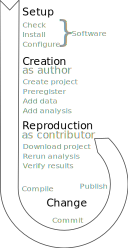
\includegraphics[width=0.5\linewidth]{images/idealized-workflow} 

}

\caption{Schematic illustration of a reproducible workflow.  }\label{fig:workflow}
\end{figure}

The structure of this chapter mirrors the workflow in Figure \ref{fig:workflow} and explains step by step how to:

\begin{enumerate}
\def\labelenumi{\arabic{enumi}.}
\tightlist
\item
  Set up the required software;
\item
  reproduce an analysis that follows the here outlined standards;
\item
  apply and publish changes;
\item
  create a reproducible workflow from scratch.
\end{enumerate}

\texttt{repro} supports several alternative software implementations for each step and integrates them into one coherent workflow.
This modular structure is inspired by the \href{https://usethis.r-lib.org}{usethis-package} (Wickham \& Bryan, \protect\hyperlink{ref-R-usethis}{2020}).
The steps described here follow the recommendations of Peikert \& Brandmaier (\protect\hyperlink{ref-peikertReproducibleDataAnalysis2019}{2019}), and hence combine RMarkdown, Git \& GitHub, Make and Docker.

\hypertarget{setup}{%
\subsection{Setup}\label{setup}}

Reproduction, change, and creation of an analysis require the user to have software installed that is specific to the workflow they choose, but independent of the analysis.
A set of functions (following the pattern \texttt{check\_*}, for a complete list see \texttt{help(check)}) assists users to ensure that everything they need is installed and correctly configured.
If \texttt{repro} detects that something is not installed or configured, it guides users through a step by step procedure on how to resolve these issues in accordance with their specific software platform.
Currently, it supports all major operating systems (Windows, OS X, Linux).

First users have to install \texttt{repro}. The following code snippet installs repro from \href{https://github.com/aaronpeikert/repro}{GitHub}:

\begin{Shaded}
\begin{Highlighting}[]
\CommentTok{# check if remotes is installed, if not install it}
\ControlFlowTok{if}\NormalTok{ (}\OperatorTok{!}\KeywordTok{requireNamespace}\NormalTok{(}\StringTok{"remotes"}\NormalTok{))\{}
  \KeywordTok{install.packages}\NormalTok{(}\StringTok{"remotes"}\NormalTok{)}
\NormalTok{\}}
\CommentTok{# install repro}
\CommentTok{# "package::function" means to use a function}
\CommentTok{# without loading the whole package}
\NormalTok{remotes}\OperatorTok{::}\KeywordTok{install_github}\NormalTok{(}\StringTok{"aaronpeikert/repro"}\NormalTok{)}
\end{Highlighting}
\end{Shaded}

If repro is installed one may load it via:

\begin{Shaded}
\begin{Highlighting}[]
\KeywordTok{library}\NormalTok{(}\StringTok{"repro"}\NormalTok{)}
\end{Highlighting}
\end{Shaded}

Subsequently, users can check if the required software is already installed.
The workflow by Peikert \& Brandmaier (\protect\hyperlink{ref-peikertReproducibleDataAnalysis2019}{2019}) depends on Git (and GitHub), Make, and Docker.
Consequently, the following commands check if the user has set up all the requirements:

\begin{Shaded}
\begin{Highlighting}[]
\KeywordTok{check_git}\NormalTok{()}
\end{Highlighting}
\end{Shaded}

\begin{verbatim}
## v Git is installed, don't worry.
\end{verbatim}

\begin{Shaded}
\begin{Highlighting}[]
\KeywordTok{check_make}\NormalTok{()}
\end{Highlighting}
\end{Shaded}

\begin{verbatim}
## v Make is installed, don't worry.
\end{verbatim}

\begin{Shaded}
\begin{Highlighting}[]
\KeywordTok{check_docker}\NormalTok{()}
\end{Highlighting}
\end{Shaded}

\begin{verbatim}
## v You are inside a Docker container!
\end{verbatim}

\begin{Shaded}
\begin{Highlighting}[]
\CommentTok{# check_github() renders this document irreproducible}
\CommentTok{# because it relies on user settings unavailable in the container}
\CommentTok{# hence it is not evaluated}
\KeywordTok{check_github}\NormalTok{()}
\end{Highlighting}
\end{Shaded}

If everything is set up, users can proceed to reproduce an analysis that conforms to this workflow.

If not, e.g.~because Docker is not installed, users get an informative message appropriate for their platform (the following code chunk shows the message windows users get when Git is missing).

\begin{Shaded}
\begin{Highlighting}[]
\KeywordTok{check_git}\NormalTok{()}
\end{Highlighting}
\end{Shaded}

\begin{verbatim}
## x Git is not installed.
\end{verbatim}

\begin{verbatim}
## i We recommend Chocolately for Windows users.
\end{verbatim}

\begin{verbatim}
## x Chocolately is not installed.
\end{verbatim}

\begin{verbatim}
## * To install it, follow directions on: 
##   'https://chocolatey.org/docs/installation'
\end{verbatim}

\begin{verbatim}
## i Use an administrator terminal to install chocolately.
\end{verbatim}

\begin{verbatim}
## * Restart your computer.
\end{verbatim}

\begin{verbatim}
## * Run `choco install -y git` in an admin terminal to install Git.
\end{verbatim}

\hypertarget{reproduction}{%
\subsection{Reproduction}\label{reproduction}}

Because this document complies with outlined requirements, it will function as an example to reproduce.
However, another more minimal example that actually contains an data analysis will be provided in the \protect\hyperlink{creation}{Creation} section below.

GitHub, Make, and Docker are sufficient to reproduce this very document.
So if you followed the steps above, everything is set up to download the source files of this document, rerun the code within it, and verify its results.

The following command uses Git and GitHub to:

\begin{enumerate}
\def\labelenumi{\arabic{enumi}.}
\tightlist
\item
  create a copy of the project, called ``fork'', in your GitHub account;
\item
  download this copy to your computer, and
\item
  verify that all files are intact and open them in a new RStudio instance.
\end{enumerate}

\begin{Shaded}
\begin{Highlighting}[]
\NormalTok{usethis}\OperatorTok{::}\KeywordTok{create_from_github}\NormalTok{(}\StringTok{"aaronpeikert/repro-thesis"}\NormalTok{,}
                            \KeywordTok{tempdir}\NormalTok{(),}
                            \DataTypeTok{fork =} \OtherTok{TRUE}\NormalTok{)}
\end{Highlighting}
\end{Shaded}

If executed, this code opens a new R session and therefor, all code from here on out needs to run in the \emph{new} session.

It is tempting to automate the reproduction part entirely and use a \texttt{rerun()} function that figures out what to do and does so for you.
However, I decided the reproduction must be feasible without the \texttt{repro} package.
This decision is supposed to ensure that long term reproducibility does not depend on the availability of the package.
I am confident that Git, Make, Docker will be available for years to come, whereas I cannot say the same about this package.
To balance the needs of long term support and usability, \texttt{repro} offers advice about what to do, but stops right before doing it.

Which steps one has to take, depends on the tools chosen to implement dependency management.
This tool determines the ``entry point'' for an analysis.
To detect the entry point, \texttt{repro} follows simple heuristics, which are informed by what most R users tend to use.
These conventions are quite ambiguous, but the clearest entry point is a \texttt{Makefile}.
If no \texttt{Makefile} is available, the alternatives are either a central dynamic document (RMarkdown, Jupityer Notebook) or a primary script (R, Python, Oktave, Shell).
In these cases, one can only guess from filenames like \texttt{manuscript.Rmd}, \texttt{analysis.Rmd}, \texttt{paper.Rmd}, \texttt{run.R} or \texttt{analysis.R}.

To recreate this document you have to follow the steps below:

\begin{Shaded}
\begin{Highlighting}[]
\CommentTok{# because this is a new R project / session, reload repro}
\KeywordTok{library}\NormalTok{(}\StringTok{"repro"}\NormalTok{)}
\KeywordTok{rerun}\NormalTok{(}\DataTypeTok{cache =} \OtherTok{FALSE}\NormalTok{)}
\end{Highlighting}
\end{Shaded}

The argument \texttt{cache\ =\ FALSE} ensures that everything that can be recreated is recreated even when nothing was changed.

It is difficult to verify wether an analysis was reproduced.
As a minimum standard one could demand, that the analysis is rerun errorfree or, as a maximal standard, that the resulting documents are exactly the same.
Neither solution strikes the right balance, because error-free does not imply the same results. At the same time the comparison of binary files often leads to spurious differences.
Currently, researchers need to revert to manual checking and common sense to verify a successful reproduction.
An automated verification procedure would require the researcher to explicitly state which results need to be identical.
Then a software solution could track changes for only these digital objects and accordingly flag mismatches.

\hypertarget{change}{%
\subsection{Change}\label{change}}

For a researcher, reproducing an analysis and verifying its results, is often only a first step to make intentional changes.
How researchers contribute to a project lays strictly outside the realm of reproducibility, but warrants discussion because easy collaboration is one of the biggest practical advantages of reproducibility.
That the primary beneficiary of this advantage is the researcher collaborating with its past self is a pun in the open science community that bears some truth.
However, the workflow of an external researcher contributing is more complicated and hence here described.
It is quite a challenge to collaborate under the circumstances where people do not work side by side or even know each other.
The core challenge is to allow the original creator full control over changes without burdening them too much.
This problem confronted the open software community from its very beginning, and they came up with the following solution.
A contributor first creates a public copy, makes and tracks changes to it and then asks the original owner to incorporate the changes.
In the terminology of GitHub, the public copy is a ``fork'', the tracked changes are ``commits'', and the call for including the changes is a ``pull request''.

Working with pull requests is easy, thanks to the \texttt{usethis} package.
If you reproduced this document, you could make changes to it---which could be something trivial, like correcting spelling---and ask me to incorporate them.
You can initialize a pull request with:

\begin{Shaded}
\begin{Highlighting}[]
\NormalTok{usethis}\OperatorTok{::}\KeywordTok{pr_init}\NormalTok{()}
\end{Highlighting}
\end{Shaded}

Subsequently, you may change the files of this thesis as you like and track them with Git.
You should make sure that the analysis is still reproducible with:

\begin{Shaded}
\begin{Highlighting}[]
\KeywordTok{rerun}\NormalTok{()}
\end{Highlighting}
\end{Shaded}

If you are satisfied with the changes you made, you can trigger the pull request with:

\begin{Shaded}
\begin{Highlighting}[]
\NormalTok{usethis}\OperatorTok{::}\KeywordTok{pr_push}\NormalTok{()}
\end{Highlighting}
\end{Shaded}

If I---as the author of this document---would like to accept, I can incorporate the changes on GitHub.
If not, the changes can be discussed in the pull request or I could make amends before merging them.

Such distributed workflow allows for a much more controlled way of collaboration as opposed to mail back and forth or using cloud storage systems.
This higher level of control matches the high standards of scientific work.
However, even more important is, that this kind of collaboration scales well for many collaborators (Git was originally developed for the collaboration on the Linux kernel, where as of 2017 more than 15.000 developers contributed code (The Linux Foundation, \protect\hyperlink{ref-thelinuxfoundation2017LinuxKernel2017}{2017})).
Empirical studies require a lot of work, which is usually distributed on many shoulders.
As the authors carry the responsibility for the overall correctness, they ought to vet every single contribution.

Affirming the correctness of a contribution can be partly automated by affirming successful reproduction.
Such automatic checks of changes are part of a software developing process, called continuous integration.
Continuous integration runs code in cloud computing environments that asserts the correctness, when changes are pushed to GitHub.
In many ways, continuous integration is the logical next step for reproducible workflows.
Because much effort was already invested in ensuring reproducibility across machines, it is easy to move the analysis to a continuous integration tool.

Hence, if you created a pull request, the continuous integration tool GitHub actions, will rebuild this document, affirming reproducibility and let me see the results of your changes.

\hypertarget{creation}{%
\subsection{Creation}\label{creation}}

Reproducing an analysis and creating a reproducible analysis are two very different issues.
The \texttt{repro} packages main strength lies in simplifying the creation.
First, the repro package comes along with a minimal, but comprehensive template including an example RMarkdown, R-script and data.
This template can be accessed from within RStudio © via ``File'' → ``New Project'' → ``New Directory'' → ``Example repro template'', or from any R console via:

\begin{Shaded}
\begin{Highlighting}[]
\KeywordTok{use_repro_template}\NormalTok{(}\StringTok{"path/to/new/project/"}\NormalTok{)}
\end{Highlighting}
\end{Shaded}

\texttt{repro} infers the dependencies to data and external code as well as the required packages from the \texttt{yaml} metadata of the RMarkdowns.
Because analytic data projects have a particular structure, this markup can be much simpler than writing \texttt{Dockerfiles} and \texttt{Makefiles} manually.
While Docker allows to install arbitrary Software, an analysis in R likely needs nothing but R-packages. Similarly, Make enables you to run any software, but an analysis in R only needs to execute R-Scripts and render RMarkdowns.

Hence, a minimal addition to the metadata, as can be seen in the following example, contains everything necessary to infer a complete \texttt{Dockerfile} and \texttt{Makefile}:

\begin{Shaded}
\begin{Highlighting}[]
\FunctionTok{repro:}
  \FunctionTok{packages:}
    \KeywordTok{-}\NormalTok{ usethis}
    \KeywordTok{-}\NormalTok{ fs}
    \KeywordTok{-}\NormalTok{ aaronpeikert/repro@d09def75df}
  \FunctionTok{scripts:}
    \KeywordTok{-}\NormalTok{ R/clean.R}
  \FunctionTok{data:}
    \FunctionTok{mycars:}\AttributeTok{ data/mtcars.csv}
\end{Highlighting}
\end{Shaded}

From this specification the function \texttt{automate()} creates a \texttt{Dockerfile} and a \texttt{Makefile}, which comply with all recommendations by Peikert \& Brandmaier (\protect\hyperlink{ref-peikertReproducibleDataAnalysis2019}{2019}).
Strictly speaking, it creates four Dockerfiles and three Makefiles.
Most of the files are created in the \texttt{.repro} directory and then assembled into the main \texttt{Dockerfile}/\texttt{Makefile} at top-level.
One \texttt{Dockerfile} contains the base docker image, including the R version and the current date and another \texttt{Dockerfile} contains only the R packages.
It also produces one file where the user can amend software installation or set up steps that are not covered by \texttt{repro}.
The \texttt{Makefiles} are similarly separated, with one file dedicated to RMarkdowns and another one for the required logic that executes the make commands in the container.

The \texttt{automate()} function is designed to simplify the workflow proposed by Peikert \& Brandmaier (\protect\hyperlink{ref-peikertReproducibleDataAnalysis2019}{2019}) as much as possible.
Such simplification means inevitably to restrict the users freedom.
While they can still do everything they want in the realm of Make and Docker, this approach does not allow other reproducibility software to be used.
Users, which need more control and are more advanced, could instead rely on the modular nature of \texttt{repro}.
Each component can be added to the project by the \texttt{use\_*} functions.
E.g. \texttt{use\_make()} adds a basic \texttt{Makefile} or \texttt{use\_make\_singularity()} adds a Makefile that is compatible with Singularity (which is an alternative to Docker for High-Performance Computing).
These functions extend the \href{https://usethis.r-lib.org}{usethis-package} (Wickham \& Bryan, \protect\hyperlink{ref-R-usethis}{2020}), which was originally designed to facilitate package development with specific reproducibility tools.

\hypertarget{summary}{%
\subsection{Summary}\label{summary}}

To summarise, if you want to create a reproducible project, you can do so with the following code:

\hypertarget{install-repro-package}{%
\subsubsection{\texorpdfstring{Install \texttt{repro} package}{Install repro package}}\label{install-repro-package}}

\begin{Shaded}
\begin{Highlighting}[]
\ControlFlowTok{if}\NormalTok{ (}\OperatorTok{!}\KeywordTok{requireNamespace}\NormalTok{(}\StringTok{"remotes"}\NormalTok{))\{}
  \KeywordTok{install.packages}\NormalTok{(}\StringTok{"remotes"}\NormalTok{)}
\NormalTok{\}}
\NormalTok{remotes}\OperatorTok{::}\KeywordTok{install_github}\NormalTok{(}\StringTok{"aaronpeikert/repro"}\NormalTok{)}
\KeywordTok{library}\NormalTok{(}\StringTok{"repro"}\NormalTok{)}
\end{Highlighting}
\end{Shaded}

\hypertarget{check-required-reproducibility-software}{%
\subsubsection{Check required reproducibility software}\label{check-required-reproducibility-software}}

\begin{Shaded}
\begin{Highlighting}[]
\KeywordTok{check_git}\NormalTok{()}
\KeywordTok{check_github}\NormalTok{()}
\KeywordTok{check_make}\NormalTok{()}
\KeywordTok{check_docker}\NormalTok{()}
\end{Highlighting}
\end{Shaded}

\hypertarget{configure-project}{%
\subsubsection{Configure Project}\label{configure-project}}

Either from template in new folder:

\begin{Shaded}
\begin{Highlighting}[]
\KeywordTok{use_repro_template}\NormalTok{(}\StringTok{"path/to/new/folder"}\NormalTok{)}
\KeywordTok{automate}\NormalTok{()}
\end{Highlighting}
\end{Shaded}

Or semi automatic with more flexibility in already existing projects:

\begin{Shaded}
\begin{Highlighting}[]
\KeywordTok{use_docker}\NormalTok{() }\CommentTok{# create Dockerfile}
\KeywordTok{use_make_docker}\NormalTok{() }\CommentTok{# create docker compatible Makefile}
\NormalTok{usethis}\OperatorTok{::}\KeywordTok{use_git}\NormalTok{() }\CommentTok{# initialize git and add first commit}
\NormalTok{rmarkdown}\OperatorTok{::}\KeywordTok{draft}\NormalTok{(}\StringTok{"pnas_article"}\NormalTok{, }\CommentTok{# use PNAS article template}
                 \DataTypeTok{package =} \StringTok{"rticles"}\NormalTok{) }\CommentTok{# requires rticles package}
\end{Highlighting}
\end{Shaded}

\hypertarget{outlook}{%
\section{Outlook}\label{outlook}}

While the \texttt{repro} package exports 33 well-documented functions, assures their correctness by close to 200 unit tests and amasses all in all short of 2000 lines of code, many workflows and features are incomplete.
I hope to make progress in three areas:

\begin{enumerate}
\def\labelenumi{\arabic{enumi}.}
\tightlist
\item
  Building an infrastructure for other workflows,
\item
  explore ``continues integration'' (CI) for research projects, and
\item
  enable the leverage of high-performance computing (HPC) clusters and cloud infrastructure.
\end{enumerate}

Because the user interface of \texttt{repro} was modeled after the \texttt{usethis} package, \texttt{repro} also inherited \texttt{usethis}' modular structure.
This design decision was made more by accident than by intention but is in hindside more than useful.
Because of its modularity, \texttt{repro} can be extended easily and can serve as an infrastructure package.
This use-case will be explored in collaboration with Caspar van Lissa, who proposes a workflow, called \href{https://cjvanlissa.github.io/worcs/}{\texttt{worcs}} (Van Lissa et al., \protect\hyperlink{ref-vanlissaWORCSWorkflowOpen2020}{2020}), which is similar in spirit, but uses different tools.
\href{https://cjvanlissa.github.io/worcs/}{\texttt{worcs}} also utilizes RMarkdown and Git, but in place of Docker, it uses \href{https://rstudio.github.io/renv/articles/renv.html}{\texttt{renv}} and instead of Make it relies on a highly standardized file structure.
Hence, only two ``moduls'' or rather functions have to be added to \texttt{repro} to support the workflow, \texttt{use\_renv()} (which replaces \texttt{use\_docker()}) and \texttt{use\_worcs\_template()} (which replaces \texttt{use\_repro\_template()}).
Also, \href{https://cjvanlissa.github.io/worcs/}{\texttt{worcs}} has other features like automatic codebook creation and synthetic data generation, which may be excellent supplements for a \texttt{repro} project.
To ensure interoperability between the packages, it is planned that much of the behind the scenes machinery is moved from \href{https://cjvanlissa.github.io/worcs/}{\texttt{worcs}} to \texttt{repro} in a more modular form.
However, the users will not notice much of a difference, except that they may fuse both workflows into one.

Such lego system of reproducibility tools, where the users can decide which tools they want to include may be especially useful when some features are not strictly necessary for reproducibility.
In its current form, no tool is optional in the sense that only in unison they guarantee reproducibility.
However, some features may be useful but not necessary for reproducibility.

For example, is it useful to have an online service such as GitHub Actions that asserts reproducibility of each change, but it is by no means necessary.
As previously discussed there currently exists no easy solution to verify reproduction automatically.
The key difficulty is to detect changes in the results that potentially alter the conclusion, from those which carry no meaning, e.g.~if the date is updated.
To address this challenge, I currently work on a prototype of an R package, which allows the researcher to assert that some objects remain unchanged upon reproduction, by wrapping them into \texttt{unchanged()}.
This package keeps track of thus marked objects and throws an error if they accidentally change.
If such a solution would exist, there would be no hurdle to incorporate continues integration into research projects.
This would mean that all contributions are automatically vetted before they are incorporated and that the results are automatically updated, e.g.~the preprint or the additional material on \url{osf.org} would automatically be re-uploaded.
Then projects could have a badge that signifies that a third party is able to reproduce it.
Such continues updates do not only ease collaboration but are also especially interesting for some continues data sources, e.g.~long-running developmental studies or meta-analysis, where new data becomes repeatedly available even after publication.

Conveniences such as the above are possible because the here presented conception of reproducibility is highly automated.
Hence, an analysis may be moved to another machine without manual intervention.
This also opens some interesting possibilities unrelated to reproducibility, concerning the management of computational resources.
It is often the case that an analysis requires substantial amounts of computational resources, more than a single computer may deliver.
In such a case, a here described analysis can easily be moved to a more powerful computer or even spread across hundreds.
The use of containers is the de facto standard of cloud computing providers but also becomes increasingly common for high-performance clusters.
Hence it is a task that can easily be accomplished with \texttt{repro}.
However, these functions are still in development and not tested well enough to be published.
A typical problem, when utilizing distributed computation, is the division of tasks between the computing instances.
However, this is pretty straightforward because of the deployed dependency management.
Make can distribute tasks across thousands of nodes while making sure that none of the dependencies collide.
Initially, this functionality was available in \texttt{repro} for TORQUE, an HPC task scheduler, but because TORQUE will no longer be maintained I will phase out this set of functions.

\texttt{repro} strives to make reproducibility more attractive by lowering the barriers to advanced reproducibility tools.
To my knowledge, no standard is as comprehensive as the here described combination of Git, RMarkdown, Make and Docker.
However, the workflow presented by Van Lissa et al. (\protect\hyperlink{ref-vanlissaWORCSWorkflowOpen2020}{2020}) sacrifices a little bit of this flexibility to reduce the complexity drastically.
Despite these efforts to make reproducibility easier, I think it is worthwhile to simplify the approaches further, to appeal to users that are more comfortable using Microsoft Office than RMarkdown and hesitant to use a formal version control system.
Hopefully, \texttt{repro} is a first step to make reproducibility easier to archive.

\hypertarget{references}{%
\section*{References}\label{references}}
\addcontentsline{toc}{section}{References}

\hypertarget{refs}{}
\leavevmode\hypertarget{ref-andersonScientificMethod2016}{}%
Andersen, H., \& Hepburn, B. (2016). Scientific method. In E. N. Zalta (Ed.), \emph{The stanford encyclopedia of philosophy} (Summer 2016). \url{https://plato.stanford.edu/archives/sum2016/entries/scientific-method/}; Metaphysics Research Lab, Stanford University.

\leavevmode\hypertarget{ref-AnnouncementReducingOur2013}{}%
Announcement: Reducing Our Irreproducibility. (2013). \emph{Nature}, \emph{496}(7446), 398--398. \url{https://doi.org/10.1038/496398a}

\leavevmode\hypertarget{ref-boultonScienceOpenEnterprise2012}{}%
Boulton, G., Campbell, P., Collins, B., Elias, P., Hall, W., Laurie, G., O'Neill, O., Rawlins, M., Thornton, J., \& Vallance, P. (2012). Science as an open enterprise. \emph{The Royal Society}.

\leavevmode\hypertarget{ref-claerboutElectronicDocumentsGive1992}{}%
Claerbout, J. F., \& Karrenbach, M. (1992). Electronic documents give reproducible research a new meaning. \emph{SEG Technical Program Expanded Abstracts 1992}, 601--604. \url{https://doi.org/10.1190/1.1822162}

\leavevmode\hypertarget{ref-dfg2019}{}%
Deutsche Forschungsgemeinschaft. (2019). \emph{Leitlinien zur Sicherung guter wissenschaftlicher Praxis}. \url{https://www.dfg.de/download/pdf/foerderung/rechtliche_rahmenbedingungen/gute_wissenschaftliche_praxis/kodex_gwp.pdf}

\leavevmode\hypertarget{ref-epskamp2019rep}{}%
Epskamp, S. (2019). Reproducibility and replicability in a fast-paced methodological world. \emph{Advances in Methods and Practices in Psychological Science}, \emph{2}(2), 145--155. \url{https://doi.org/https://doi.org/10.1177/2515245919847421}

\leavevmode\hypertarget{ref-gigerenzerNullRitualWhat2004}{}%
Gigerenzer, G., Krauss, S., \& Vitouch, O. (2004). The Null Ritual: What You Always Wanted to Know About Significance Testing but Were Afraid to Ask. In D. Kaplan, \emph{The SAGE Handbook of Quantitative Methodology for the Social Sciences} (pp. 392--409). SAGE Publications, Inc. \url{https://doi.org/10.4135/9781412986311.n21}

\leavevmode\hypertarget{ref-gilbertModelBuildingDefinition1991}{}%
Gilbert, S. W. (1991). Model building and a definition of science. \emph{Journal of Research in Science Teaching}, \emph{28}(1), 73--79. \url{https://doi.org/10.1002/tea.3660280107}

\leavevmode\hypertarget{ref-heilbronOxfordCompanionHistory2004}{}%
Heilbron, J. L. (Ed.). (2004). The Oxford Companion to the History of Modern Science. \emph{Reference Reviews}, \emph{18}(4), 40--41. \url{https://doi.org/10.1108/09504120410535443}

\leavevmode\hypertarget{ref-hutsonArtificialIntelligenceFaces2018}{}%
Hutson, M. (2018). Artificial intelligence faces reproducibility crisis. \emph{Science}, \emph{359}(6377), 725--726. \url{https://doi.org/10.1126/science.359.6377.725}

\leavevmode\hypertarget{ref-ioannidisWhyMostPublished2005}{}%
Ioannidis, J. P. A. (2005). Why Most Published Research Findings Are False. \emph{PLOS Medicine}, \emph{2}(8), e124. \url{https://doi.org/10.1371/journal.pmed.0020124}

\leavevmode\hypertarget{ref-jordanMachineLearningTrends2015}{}%
Jordan, M. I., \& Mitchell, T. M. (2015). Machine learning: Trends, perspectives, and prospects. \emph{Science}, \emph{349}(6245), 255--260. \url{https://doi.org/10.1126/science.aaa8415}

\leavevmode\hypertarget{ref-krakerCaseOpenScience2011}{}%
Kraker, P., Leony, D., Reinhardt, W., Gü, N., \& Beham, nter. (2011). The case for an open science in technology enhanced learning. \emph{International Journal of Technology Enhanced Learning}, \emph{3}(6), 643. \url{https://doi.org/10.1504/IJTEL.2011.045454}

\leavevmode\hypertarget{ref-martinCleanCoderCode2011}{}%
Martin, R. C. (2011). \emph{The clean coder: A code of conduct for professional programmers / Robert C. Martin} (1. print.). Prentice Hall.

\leavevmode\hypertarget{ref-maxwellPsychologySufferingReplication2015}{}%
Maxwell, S. E., Lau, M. Y., \& Howard, G. S. (2015). Is psychology suffering from a replication crisis? What does ``failure to replicate'' really mean? \emph{American Psychologist}, \emph{70}(6), 487.

\leavevmode\hypertarget{ref-meehlAppraisingAmendingTheories1990}{}%
Meehl, P. E. (1990). Appraising and Amending Theories: The Strategy of Lakatosian Defense and Two Principles that Warrant It. \emph{Psychological Inquiry}, \emph{1}(2), 108--141. \url{https://doi.org/10.1207/s15327965pli0102_1}

\leavevmode\hypertarget{ref-meehlTheoreticalRisksTabular1978}{}%
Meehl, P. E. (1978). Theoretical risks and tabular asterisks: Sir Karl, Sir Ronald, and the slow progress of soft psychology. \emph{Journal of Consulting and Clinical Psychology}, \emph{46}(4), 806--834. \url{https://doi.org/10.1037/0022-006X.46.4.806}

\leavevmode\hypertarget{ref-R-here}{}%
Müller, K. (2017). \emph{Here: A simpler way to find your files}. \url{https://CRAN.R-project.org/package=here}

\leavevmode\hypertarget{ref-nosekPreregistrationRevolution2018}{}%
Nosek, B. A., Ebersole, C. R., DeHaven, A. C., \& Mellor, D. T. (2018). The preregistration revolution. \emph{Proceedings of the National Academy of Sciences}, \emph{115}(11), 2600--2606. \url{https://doi.org/10.1073/pnas.1708274114}

\leavevmode\hypertarget{ref-nuijtenPrevalenceStatisticalReporting2016}{}%
Nuijten, M. B., Hartgerink, C. H. J., van Assen, M. A. L. M., Epskamp, S., \& Wicherts, J. M. (2016). The prevalence of statistical reporting errors in psychology (1985--2013). \emph{Behavior Research Methods}, \emph{48}(4), 1205--1226. \url{https://doi.org/10.3758/s13428-015-0664-2}

\leavevmode\hypertarget{ref-opensciencecollaborationEstimatingReproducibilityPsychological2015}{}%
Open Science Collaboration. (2015). Estimating the reproducibility of psychological science. \emph{Science}, \emph{349}(6251), aac4716--aac4716. \url{https://doi.org/10.1126/science.aac4716}

\leavevmode\hypertarget{ref-peikertReproducibleDataAnalysis2019}{}%
Peikert, A., \& Brandmaier, A. M. (2019). \emph{A Reproducible Data Analysis Workflow with R Markdown, Git, Make, and Docker} {[}Preprint{]}. PsyArXiv. \url{https://doi.org/10.31234/osf.io/8xzqy}

\leavevmode\hypertarget{ref-R-repro}{}%
Peikert, A., Brandmaier, A. M., \& van Lissa, C. J. (2020). \emph{Repro: Automated setup of reproducible workflows and their dependencies}. \url{https://github.com/aaronpeikert/repro}

\leavevmode\hypertarget{ref-popperCommentsTruthGrowth1962}{}%
Popper, K. R. (1962). Some comments on truth and the growth of knowledge. In E. Nagel, P. Suppes, \& A. Tarski (Eds.), \emph{Logic, Methodology and Philosophy of Science Proceedings of the 1960 International Congress} (Vol. 155). Stanford University Press.

\leavevmode\hypertarget{ref-R-base}{}%
R Core Team. (2020). \emph{R: A language and environment for statistical computing}. R Foundation for Statistical Computing. \url{https://www.R-project.org/}

\leavevmode\hypertarget{ref-rodgersEpistemologyMathematicalStatistical2010}{}%
Rodgers, J. L. (2010). The epistemology of mathematical and statistical modeling: A quiet methodological revolution. \emph{American Psychologist}, \emph{65}(1), 1--12. \url{https://doi.org/10.1037/a0018326}

\leavevmode\hypertarget{ref-thelinuxfoundation2017LinuxKernel2017}{}%
The Linux Foundation. (2017, October 25). \emph{2017 Linux Kernel Report Highlights Developers' Roles and Accelerating Pace of Change}. \url{https://www.linuxfoundation.org/blog/2017/10/2017-linux-kernel-report-highlights-developers-roles-accelerating-pace-change/}

\leavevmode\hypertarget{ref-theturingwaycommunityTuringWayHandbook2019}{}%
The Turing Way Community, Arnold, B., Bowler, L., Gibson, S., Herterich, P., Higman, R., Krystalli, A., Morley, A., O'Reilly, M., \& Whitaker, K. (2019). \emph{The Turing Way: A Handbook for Reproducible Data Science}. \url{https://doi.org/10.5281/zenodo.3233986}

\leavevmode\hypertarget{ref-tichyVerisimilitudeRedefined1976}{}%
Tichỳ, P. (1976). Verisimilitude redefined. \emph{The British Journal for the Philosophy of Science}, \emph{27}(1), 25--42.

\leavevmode\hypertarget{ref-vanlissaWORCSWorkflowOpen2020}{}%
Van Lissa, C. J., Brandmaier, A. M., Brinkman, L., Lamprecht, A.-L., Peikert, A., Struiksma, M., \& Vreede, B. (2020). \emph{WORCS: A Workflow for Open Reproducible Code in Science} {[}Preprint{]}. PsyArXiv. \url{https://doi.org/10.31234/osf.io/k4wde}

\leavevmode\hypertarget{ref-R-usethis}{}%
Wickham, H., \& Bryan, J. (2020). \emph{Usethis: Automate package and project setup}. \url{https://CRAN.R-project.org/package=usethis}

\leavevmode\hypertarget{ref-williamsStyleLessonsClarity2017}{}%
Williams, J. M. (2017). \emph{Style: Lessons in clarity and grace} (Twelfth Edition). Pearson.

\leavevmode\hypertarget{ref-xieMarkdownDefinitiveGuide2019}{}%
Xie, Y., Allaire, J. J., \& Grolemund, G. (2019). \emph{R Markdown: The definitive guide}.

\end{document}
